\chapter{Results and Discussion}
\label{chap:discussion}

% \section{Results}
% \label{sec:results}

Due to the interdisciplinary nature of this work the results can be analysed from several different perspectives. We start with a quantitative analysis of the pointing precision in the experiment, defined by the Euclidean distance metric. The performance of the two models implemented in the robot is compared in terms of the lowest pointing errors. Then, we focus on the implications of the model and its results for neuroscience, developmental psychology and cognitive robotics. Finally, we discuss possible extensions and improvements of the model and the experimental setting by proposing future research directions.



\section{Quantitative Analysis}

In this section we compare the robot's hand trajectory and the trajectory representing positions of the object held by the experimenter throughout the experiment. 
Ideally, one would like to see overlapping between the two trajectories, but since the object was sometimes out of reach of robot's hand, whose length was 240 mm in total, the robot could physically not reach these positions. Thus, for the purposes of comparison we are primarily interested in analysing the direction of pointing along a given axis.
The 3D position of the marker was taken as a ground truth in the attempt to evaluate the precision of pointing. 
Positions of the marker and the robot's hand are plotted over one second of the experiment and along all three dimensions in Figure \ref{lab:trajectory_x}.
The red line represents the hand position as determined by the \ssom model and the green one the hand position as determined by the \bsom model. We see that both trajectories approximately follow the blue line, which is the position of the object.
The green line is characterised by a higher resolution, which is expected because the greater number of neurons is responsible for greater number of possible arm postures.

\begin{figure}[ht!]
\vspace*{-3cm}
\centering
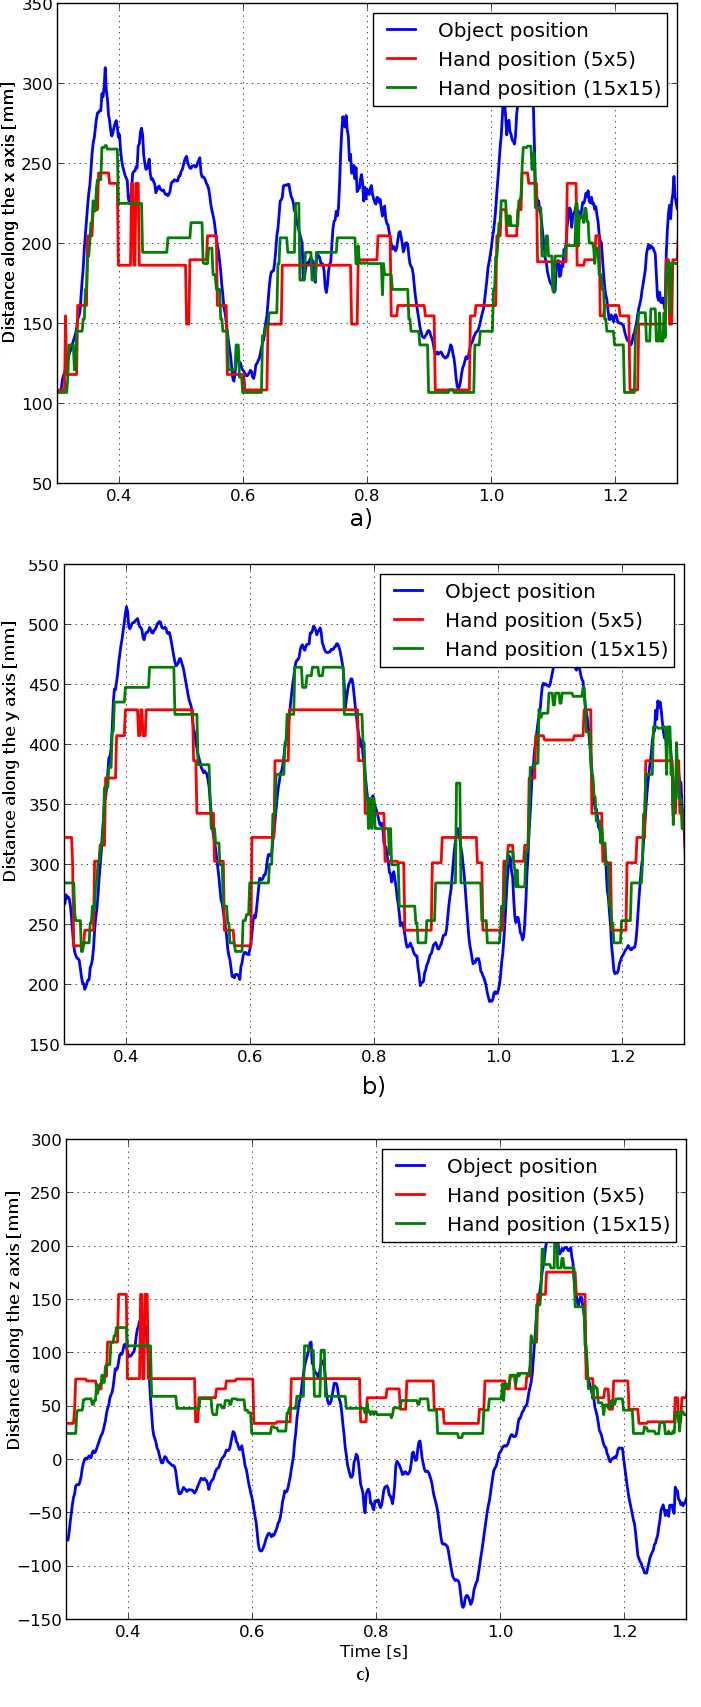
\epsfig{file=merged_trajectories_1.png, height=23cm}
\caption{Left hand trajectory along horizontal (a), vertical (b) and depth (c) axis as predicted by the two models and the ground truth value}
\label{lab:trajectory_x}
\end{figure}


% \begin{figure}[t]
% \centering
% \epsfig{file=trajectory_x1.png, height=8cm}
% \caption{Left hand trajectory along the horizontal axis as predicted by the two models and the ground truth value}
% \label{lab:trajectory_x}
% \end{figure}
% 
% \begin{figure}
% \centering
% \epsfig{file=trajectory_z1.png, height=8cm}
% \caption{Left hand trajectory along the vertical axis as predicted by the two models and the ground truth value}
% \label{lab:trajectory_y}
% \end{figure}
% 
% \begin{figure}
% \centering
% \epsfig{file=trajectory_y1.png, height=8cm}
% \caption{Left hand trajectory along the depth axis as predicted by the two models and the ground truth value}
% \label{lab:trajectory_z}
% \end{figure}

As a simple quantification measure of pointing we introduced the pointing precision error, which is defined as the Euclidean distance between the position of a marker and the hand position. A paired-samples t-test was conducted to compare precision errors for the $5\times 5$ network and the $15 \times 15$ network. There was a significant improvement in the performances from the $5 \times 5$ network ($Mean\ error=99.93mm$
, $Std.\ Dev.=32.10$) to the $15 \times 15$ network ($Mean\ error=80.32mm$, $Std.\ Dev.=33.41$) conditions; $t(1400)=76.47$, $p<0.05$. It is important to mention once again that the high error is the result of the difference between the maximal arm length and the unreachable object positions. 


\section{Implications of the Model}
With this work an important open question ``How can pointing emerge from grasping behaviour'' (T2.3 from \citep{Kaplan2006}) in developmental psychology and developmental robotics has been addressed. We identified and extended the informational and sensory prerequisites for realising pointing from motor babbling in a computational model. Compared to a similar model presented in \citep{SchillaciH11}, the advantage of our model is the biological plausibility, which aims to make a contribution towards the research in neuroscience and robotics. The modular organisation of the model in terms of sensory maps and associated representations of sensory data via Hebbian learning allows for easier extension and identification of its components with the biological equivalents. It has to be pointed out that the biologically inspired model has not been adopted just for the sake of reproducing a biological system into an artificial one. Rather, our aim is to provide the robot with capabilities such as autonomous learning, 
adaptability and plasticity. In fact, state-of-the-art robots still lack basic capabilities such as learning, adapting, reacting to unexpected circumstances, exhibiting a proper level of intelligence and autonomously and safely operating in unconstrained and uncertain environments.

Through the proposed SOM-model a robot can autonomously build up an internal representation of its body, or of parts of it. In particular, the nature of the proposed model allows an artificial agent to build up and, eventually, to reshape its internal body representation through the interaction with the external world.
In addition, a particular emphasis has been given to the developmental progression in the acquisition of motor and cognitive skills (such as attention manipulation through pointing gestures). We strongly believe that studying human development could give insights in finding those basic behavioural components that may allow for an autonomous mental and motor development in artificial agents. A robot capable of developing motor and mental skills autonomously can better deal with the aforementioned challenges related to real world scenarios.


Moreover, the results enable us to draw several parallels with respect to the development of pointing skills in infants. First, the two instances of the model can be compared to the two different stages of hand-eye coordination development. Under the assumption that the more advanced stage is described by more specialised neurons which facilitate pointing, the model containing more neurons simulates the later stage by performing significantly better in terms of smaller pointing errors. Second, we explored the influence of the data acquisition procedure through random motor babbling and showed that longer babbling phases yield better pointing accuracies. Following this line of arguments, one would expect that infants which explored a larger set of body configurations might acquire better manual coordination. This hypothesis can be further tested by analysing the motor coordination of children who were differently exposed to sports in their early childhood. 

When trained on different data, the model for pointing can be used for learning 
other sensorimotor skills. For example, one could use the model to learn 
relations between observed pointing gestures and motor commands for moving into 
the pointed direction, similarly to \citep{Bodiroza2013}. Knowing and handling 
these relations is important, as situations requiring them occur in everyday 
life. For example, in a bookstore when we point to a book on a shelf we cannot 
reach or on the street where we ask for an unknown path. Thus, for robots to 
exhibit human-like behaviour in such situations they need to be able to 
recognize the pointed position and to associate this position with a certain 
motor command which should be issued to reach that position. In order to achieve 
this behaviour, one would need to train one SOM to represent the space of joint 
configurations and associate this SOM with the motor commands in the second SOM. 
Depending on whether the robot should point or move, one should use one or the 
other 
SOM to guide the kinematics of the robot.


